% macro_usage_guide.tex
% Complete overzicht van alle school-macros features

\documentclass[a4paper,11pt]{article}
\usepackage{school-macros}

\title{School Macros — Volledige Gids}
\author{Macro Voorbeelden}
\date{\today}

\begin{document}

\maketitle
\tableofcontents
\newpage

\section{Box Macros}

\subsection{Examenbox (Compact Stijl)}
\begin{examenbox}
Dit is een examentip in compacte vorm. Gebruik dit voor korte, praktische tips voor examens.
Let op: deze heeft geen titel parameter nodig.
\end{examenbox}

\subsection{Conceptbox}
\begin{conceptbox}[title=Belangrijke Definitie]
\textbf{Snijsnelheid} ($v_c$): de omtrekssnelheid van het gereedschap ten opzichte van het werkstuk, gemeten in m/min.

Conceptbox heeft een grijze achtergrond met blauwe accent links.
\end{conceptbox}

\begin{conceptbox}
Je kan ook een aangepaste titel gebruiken door [title=...] mee te geven.
\end{conceptbox}

\subsection{Warningbox}
\begin{warningbox}
Zonder titel parameter (geen titel-balk bovenaan).
\end{warningbox}

\begin{warningbox}[title=CUSTOM WAARSCHUWING]
Je kan ook een aangepaste titel gebruiken door [title=...] mee te geven.
\end{warningbox}

\subsection{Oefenblok}
\begin{oefenblok}
Eenvoudige oefening zonder titel (geen titel-balk bovenaan).

Bereken de snijsnelheid als het toerental $n = 1200$ rpm en de diameter $d = 50$ mm.

\textbf{Oplossing:}
\[ v_c = \pi d n = \pi \times 0.05 \times 1200 = 188.5 \text{ m/min} \]
\end{oefenblok}

\begin{oefenblok}[title=Custom Oefening Titel]
Je kan ook een aangepaste titel gebruiken, net zoals bij conceptbox.
\end{oefenblok}

\section{Formule Macros}

\subsection{Formula box (\textbackslash frm)}
De \verb|\frm| macro creëert automatisch een formularium entry:

\frm{Snijsnelheid}{v_c = \pi d n}{waarbij $d$ de diameter in meter en $n$ het toerental in omw/min}

\frm{Vermogen}{P = F_c \cdot v_c}{$F_c$ is de snijkracht in N, $v_c$ in m/s}

\frm{Kinetische Energie}{E_k = \frac{1}{2}mv^2}{waarbij $m$ de massa [kg] en $v$ de snelheid [m/s]}

\subsection{Boxed vergelijking}
Voor belangrijke vergelijkingen in de tekst:
\[ \eqbox{E = mc^2} \]

Of gewoon:
\[ \boxed{F = ma} \]

\section{Text Emphasis}

\begin{itemize}
\item \verb|\concept{...}|: \concept{Dit is een belangrijk concept} (blauw, vet)
\item \verb|\belangrijk{...}|: \belangrijk{Dit is een belangrijke waarschuwing} (rood, vet)
\item \verb|\keyterm{...}|: \keyterm{Sleutelbegrip} (blauw accent)
\end{itemize}

\section{Math Shortcuts}

\subsection{Differentialen}
\begin{itemize}
\item \verb|\diff|: $\diff x$ (differentiaal operator)
\item \verb|\dx, \dy, \dt, \dv|: $\dx, \dy, \dt, \dv$ (voor integralen)
\item \verb|\dd{y}{x}|: $\dd{y}{x}$ (gewone afgeleide)
\item \verb|\ddn{y}{x}{2}|: $\ddn{y}{x}{2}$ (2e afgeleide)
\item \verb|\pd{f}{x}|: $\pd{f}{x}$ (partiële afgeleide)
\item \verb|\pdn{f}{x}{2}|: $\pdn{f}{x}{2}$ (2e partiële afgeleide)
\end{itemize}

Voorbeeld integraal:
\[ \int_0^1 x^2 \, \dx = \left[\frac{x^3}{3}\right]_0^1 = \frac{1}{3} \]

\subsection{Vectoren en Matrices}
\begin{itemize}
\item \verb|\vec{v}|: $\vec{v}$ (vector, vetgedrukt)
\item \verb|\uvec{x}|: $\uvec{x}$ (eenheidsvector met hoedje)
\item \verb|\mat{A}|: $\mat{A}$ (matrix)
\end{itemize}

Voorbeeld:
\[ \vec{F} = m\vec{a} \quad \text{en} \quad \uvec{n} = \frac{\vec{v}}{\norm{\vec{v}}} \]

\subsection{Verzamelingen}
\begin{itemize}
\item \verb|\RR|: $\RR$ (reële getallen)
\item \verb|\NN|: $\NN$ (natuurlijke getallen)
\item \verb|\ZZ|: $\ZZ$ (gehele getallen)
\item \verb|\QQ|: $\QQ$ (rationale getallen)
\item \verb|\CC|: $\CC$ (complexe getallen)
\end{itemize}

\subsection{Haakjes en Normen (Auto-scaling)}
\begin{itemize}
\item \verb|\abs{x}|: $\abs{x}$ (absolute waarde)
\item \verb|\norm{v}|: $\norm{v}$ (norm)
\item \verb|\paren{...}|: $\paren{\frac{a}{b}}$ (ronde haakjes)
\item \verb|\bracket{...}|: $\bracket{\frac{a}{b}}$ (vierkante haakjes)
\item \verb|\curlybrace{...}|: $\curlybrace{\frac{a}{b}}$ (accolades)
\item \verb|\avg{...}|: $\avg{x}$ (gemiddelde)
\end{itemize}

\subsection{Snelle Breuken}
\begin{itemize}
\item \verb|\half|: $\half$
\item \verb|\third|: $\third$  
\item \verb|\quarter|: $\quarter$
\item \verb|\ifrac{1}{3}|: \ifrac{1}{3} (inline text fraction: 1/3)
\end{itemize}

\section{Figuren}

\subsection{Standaard figuur (\textbackslash fig)}
Syntax: \verb|\fig[breedte]{pad}{onderschrift}{label}|

Voorbeeld (uncomment om te gebruiken):
\begin{verbatim}
\fig[0.6\linewidth]{image.png}{Een voorbeeld figuur}{fig:example}
\end{verbatim}

\subsection{Auto figuur (\textbackslash autofig)}
Genereert automatisch een label gebaseerd op de bestandsnaam:
\begin{verbatim}
\autofig[0.5\linewidth]{path/to/image.png}{Caption text}
\end{verbatim}

\subsection{Simpel image (\textbackslash img)}
Nog eenvoudiger - alleen pad en caption:
\begin{verbatim}
\img{path/to/image.png}{Caption}
\end{verbatim}

\section{Symbolen}

\subsection{Symbol registratie (\textbackslash sym)}
Bij eerste gebruik toont \verb|\sym| een box met uitleg:

\sym{v_c}{Snijsnelheid}{m/min}
\sym{F_c}{Snijkracht}{N}
\sym{P}{Vermogen}{W}
\sym{omega}{Hoeksnelheid}{rad/s}

Later in de tekst gebruik je gewoon het symbool: $v_c = 100$ m/min, $F_c = 500$ N.

Tweede gebruik toont alleen het symbool: \sym{v_c}{Snijsnelheid}{m/min}

\section{Cross-References (Nederlands)}

\begin{itemize}
\item \verb|\eqnref{eq:label}|: \eqnref{eq:example} (verwijzing naar vergelijking)
\item \verb|\Eqnref{eq:label}|: \Eqnref{eq:example} (aan begin van zin)
\item \verb|\figref{fig:label}|: verwijzing naar figuur
\item \verb|\Figref{fig:label}|: Figuur aan begin van zin
\item \verb|\tabref{tab:label}|: verwijzing naar tabel
\item \verb|\Tabref{tab:label}|: Tabel aan begin van zin
\item \verb|\secref{sec:label}|: verwijzing naar sectie
\item \verb|\Secref{sec:label}|: Sectie aan begin van zin
\end{itemize}

Voorbeeld vergelijking met label:
\begin{equation}\label{eq:example}
E = mc^2
\end{equation}

\section{Utility Macros}

\subsection{TODO markers}
\TODO{Voeg hier meer voorbeelden toe}

\FIXME{Controleer deze berekening}

\NOTE{Belangrijk om te onthouden voor het examen}

\subsection{Degree symbool}
Gebruik \verb|\degree| voor graden: $45\degree$, $90\degree$

\section{Lists met enumitem}

\subsection{Genummerde lijst}
\begin{enumerate}
\item Eerste punt
\item Tweede punt
    \begin{enumerate}
    \item Sub-punt A
    \item Sub-punt B
    \end{enumerate}
\item Derde punt
\end{enumerate}

\subsection{Bullet lijst}
\begin{itemize}
\item Eerste item
\item Tweede item
    \begin{itemize}
    \item Sub-item 1
    \item Sub-item 2
    \end{itemize}
\item Derde item
\end{itemize}

\subsection{Beschrijvingslijst}
\begin{description}
\item[Snelheid] Afgelegde afstand per tijdseenheid
\item[Versnelling] Verandering van snelheid per tijdseenheid
\item[Kracht] Het product van massa en versnelling
\end{description}

\section{Tabellen}

\subsection{Basis tabel met booktabs}
\begin{table}[H]
\centering
\caption{Materiaaleigenschappen}
\begin{tabular}{lcc}
\toprule
\textbf{Materiaal} & \textbf{Dichtheid [kg/m³]} & \textbf{E-modulus [GPa]} \\
\midrule
Staal & 7850 & 210 \\
Aluminium & 2700 & 70 \\
Beton & 2400 & 30 \\
\bottomrule
\end{tabular}
\end{table}

\subsection{Tabel met lange tekst (tabularx)}
\begin{table}[H]
\centering
\caption{Begrippen en definities}
\begin{tabularx}{\linewidth}{l X}
\toprule
\textbf{Begrip} & \textbf{Definitie} \\
\midrule
Spanning & De kracht per oppervlakte-eenheid die op een materiaal wordt uitgeoefend \\
\addlinespace
Rek & De relatieve verlenging of verkorting van een materiaal onder belasting \\
\bottomrule
\end{tabularx}
\end{table}

\section{Grafieken met TikZ/PGFPlots}

\subsection{Functie Plot}
\begin{center}
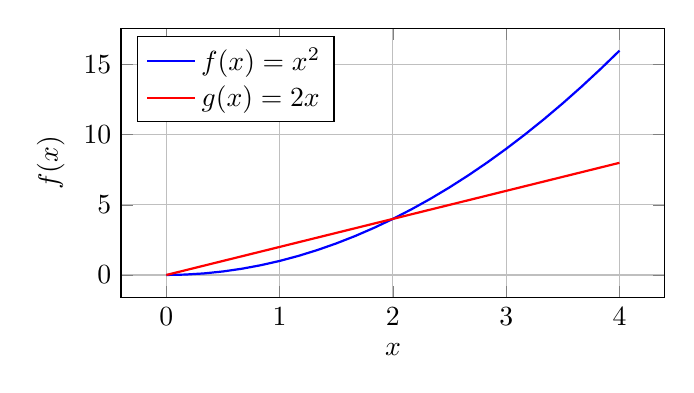
\begin{tikzpicture}
\begin{axis}[
    width=0.7\linewidth,
    height=5cm,
    xlabel={$x$},
    ylabel={$f(x)$},
    grid=major,
    legend pos=north west
]
\addplot[blue, thick, domain=0:4] {x^2};
\addlegendentry{$f(x) = x^2$}
\addplot[red, thick, domain=0:4] {2*x};
\addlegendentry{$g(x) = 2x$}
\end{axis}
\end{tikzpicture}
\end{center}

\subsection{Data Plot}
\begin{center}
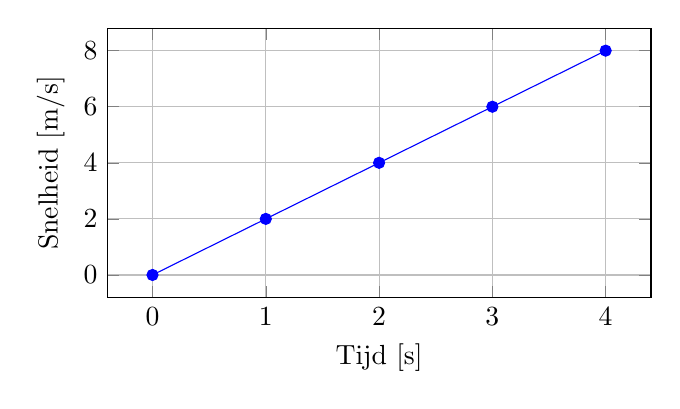
\begin{tikzpicture}
\begin{axis}[
    width=0.7\linewidth,
    height=5cm,
    xlabel={Tijd [s]},
    ylabel={Snelheid [m/s]},
    grid=major
]
\addplot[mark=*, blue] coordinates {
    (0,0) (1,2) (2,4) (3,6) (4,8)
};
\end{axis}
\end{tikzpicture}
\end{center}

\subsection{Eenvoudig TikZ Diagram}
\begin{center}
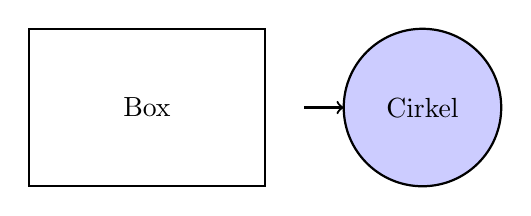
\begin{tikzpicture}
% Rechthoek
\draw[thick] (0,0) rectangle (3,2);
% Cirkel
\draw[thick, fill=blue!20] (5,1) circle (1);
% Pijl
\draw[->, thick] (3.5,1) -- (4,1);
% Tekst
\node at (1.5,1) {Box};
\node at (5,1) {Cirkel};
\end{tikzpicture}
\end{center}

\section{Geavanceerde Layout}

\subsection{Tekst naast Figuur (minipage)}
\begin{figure}[H]
    \centering
    \begin{minipage}{0.55\textwidth}
        \textbf{Uitleg bij de figuur:}
        
        Door minipage te gebruiken kun je tekst en een afbeelding naast elkaar plaatsen.
        
        Let op dat de breedtes samen niet meer dan 1.0\textbackslash textwidth zijn.
    \end{minipage}%
    \hfill
    \begin{minipage}{0.4\textwidth}
        \centering
        \fbox{Plaats hier je afbeelding}
    \end{minipage}
\end{figure}

\subsection{Multiple kolommen}
\begin{multicols}{2}
Dit is tekst in twee kolommen. Gebruik \texttt{multicols} voor automatische kolommen.

De tekst vloeit automatisch van de ene kolom naar de andere.

Je kan dit gebruiken voor compacte opsommingen of vergelijkingen.

\columnbreak

Tweede kolom begint hier. Je kan \verb|\columnbreak| gebruiken om handmatig naar de volgende kolom te gaan.
\end{multicols}

\section{Workflow Tips}

\subsection{Belangrijk}
\begin{enumerate}
\item Compileer \textbf{tweemaal} voor formularium en symbolenlijst
\item Gebruik \verb|\frm| voor alle belangrijke formules
\item Gebruik \verb|\sym| bij eerste vermelding van symbolen
\item Gebruik \verb|school-macros| package voor consistentie
\end{enumerate}

\subsection{Typisch Document Structuur}
\begin{verbatim}
\documentclass[a4paper,11pt]{article}
\usepackage{school-macros}

\title{Titel}
\author{Naam}
\date{\today}

\begin{document}
\maketitle
\tableofcontents
\newpage

\section{Hoofdstuk}
% Inhoud...

\appendix
\printsymbols
\printformularium
\end{document}
\end{verbatim}

\appendix
\section*{Symbolenlijst}
\printsymbols

\section*{Formularium}
\printformularium

\end{document}
